%
% LO, Li-yu 
%

\documentclass[a4paper,12pt]{article}

\usepackage{graphicx}
\usepackage[english]{babel}
\usepackage[]{amsmath}
\usepackage{amsfonts}
\usepackage{mathtools}
\usepackage{amssymb}
\usepackage[a4paper, portrait, margin=0.8in]{geometry}
\usepackage{hyperref}
\usepackage{algorithm,algpseudocode}
\usepackage{indentfirst}
\usepackage{soul}
\usepackage{color}
% \usepackage{subfigure}
\usepackage{titling}
% \usepackage{subcaption}
\usepackage{subfig}
\usepackage[labelfont=bf, justification=justified]{caption}
% \usepackage[demo]{graphicx}% Remove demo option in real document


\setlength{\droptitle}{-4em}   % This is your set screw

\begin{document}
%
   \title{\textbf{COMP5212 Machine Learning} \\  
   Programming Homework 2}
   
   \author{LO, Li-yu \\ 20997405 \\ e-mail: lloac@connect.hkust.hk}
   \date{\today}
   \maketitle

\vspace*{-1.2cm}
\section*{Abstract}
\vspace*{-0.4cm}
In this assignment, we aim to train a multi-class classifier on CIFAR-10 dataset
with following models:
(1) \textbf{Multi-Layer Perceptron (MLP)} and 
(2) \textbf{Convolutional Neural Network (CNN)}.
In particular, We adopt PyTorch library as our main 
programming framework. Below then reports the training results.
Note that all the training was carried on GeForce RTX 3080 Ti.
\vspace*{-0.6cm}
\section*{Multi-Layer Perceptron}
\vspace*{-0.4cm}
We first discuss the model using multi-layer perceptron. In which, 7 fully connected NN layers
are deployed with ReLU activation function. 
The input/output sizes of each layer is defined to reduce the dimension equally 
after one NN + activation layer, from initial data input size 3072 to final output size 10. 
The input/output sizes of each layer are therefore:
3072/2633, 2633/2194, 2194/1755, 1755/1316, 1316/877, 877/438, and 438/10.
As for training, we utilize SGD-M, with $learning \; rate \; \alpha=0.01$, momentum coefficient 
$\beta=0.9$ and $epoch=20$.
On the other hand, the cost function is cross-entropy. 
Below is the training results and calculated accuracy:
\vspace*{-0.6cm}
\begin{figure}[!htb]
   \captionsetup[subfigure]{justification=centering}
   \centering
   \subfloat[][MLP Loss v. Epochs]
   {%
      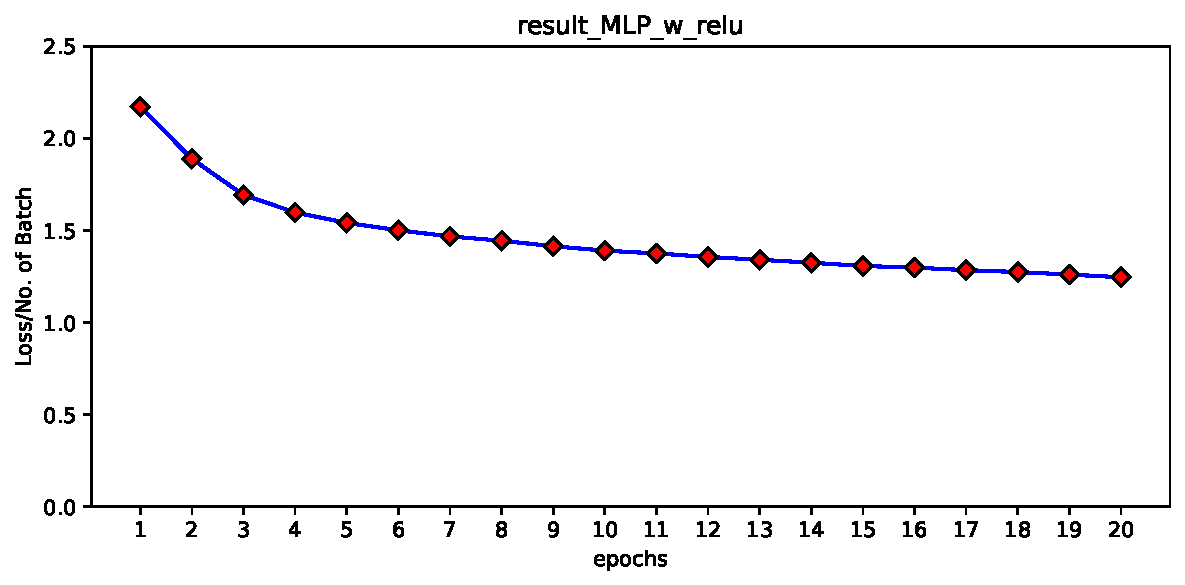
\includegraphics[width=0.45\textwidth]{./results/result_MLP_w_relu.pdf}%
      \label{fig:mlp_loss}
   }%
   \hspace{0.5cm}%
   \subfloat[][MLP Accuracy]
   {%
      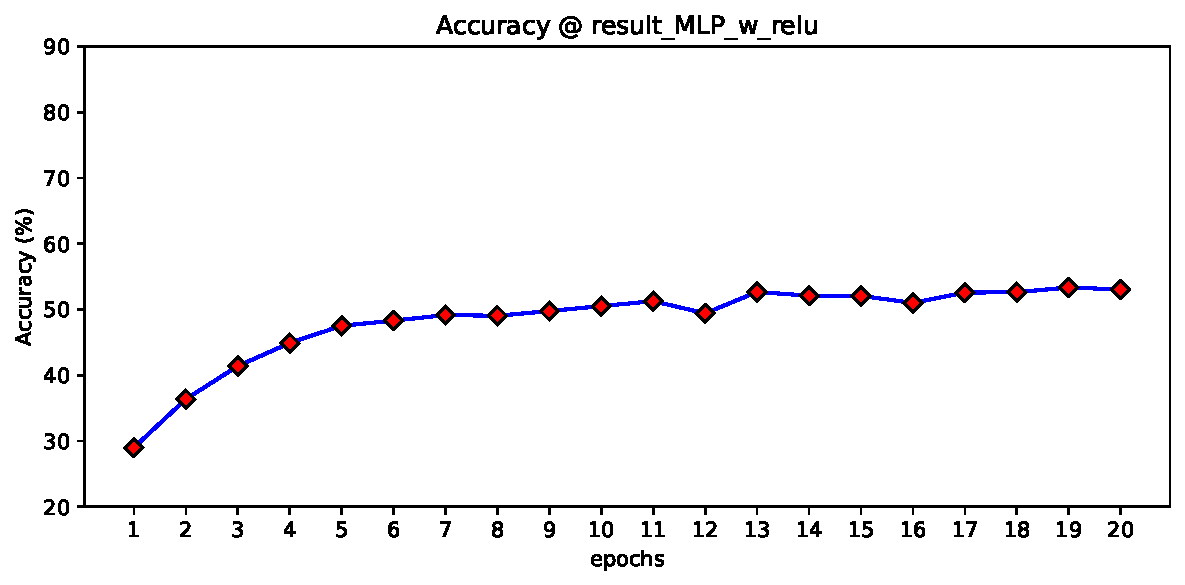
\includegraphics[width=0.45\textwidth]{./results/result_MLP_w_relu_accuracy.pdf}%
      \label{fig:mlp_acc}
   }
   \caption{Multi-Layer Perceptron training results.}
\end{figure}
\vspace*{-0.6cm}
\section*{Convolutional Neural Network}
\vspace*{-0.4cm}
As mentioned, a classifier with convolutional neural network is also trained.
In which, 4 convolutional layers and 3 fully connected layers, with ReLU activation function
is adopted. Particularly, to fulfill the training requirement, where the input size 
of $1^{st}$ fully connected layer should be 4096, each CNN layer information is as followed:
(1) 2D convolution kernel $5 \times 5$/input channel 3/output channel 66,
(2) 2D convolution kernel $5 \times 5$/input channel 66/output channel 128/stride (2,2)/padding (1,1),
(3) 2D convolution kernel $5 \times 5$/input channel 128/output channel 192,
and
(4) 2D convolution kernel $5 \times 5$/input channel 192/output channel 256/stride (2,2)/padding (1,1).
As for the fully connected layers, the input/output size of each FLC layer information 
is as followed: 4096/2734, 2734/1372, and 1372/10.
Similar to MLP, we utilize SGD-M, with $learning \; rate \; \alpha=0.01$, 
$\beta=0.9$ and $epoch=20$.
On the other hand, the cost function is cross-entropy.
Below is the training results and calculated accuracy:

\begin{figure}[!htb]
   \captionsetup[subfigure]{justification=centering}
   \centering
   \subfloat[][CNN Loss v. Epochs]
   {%
      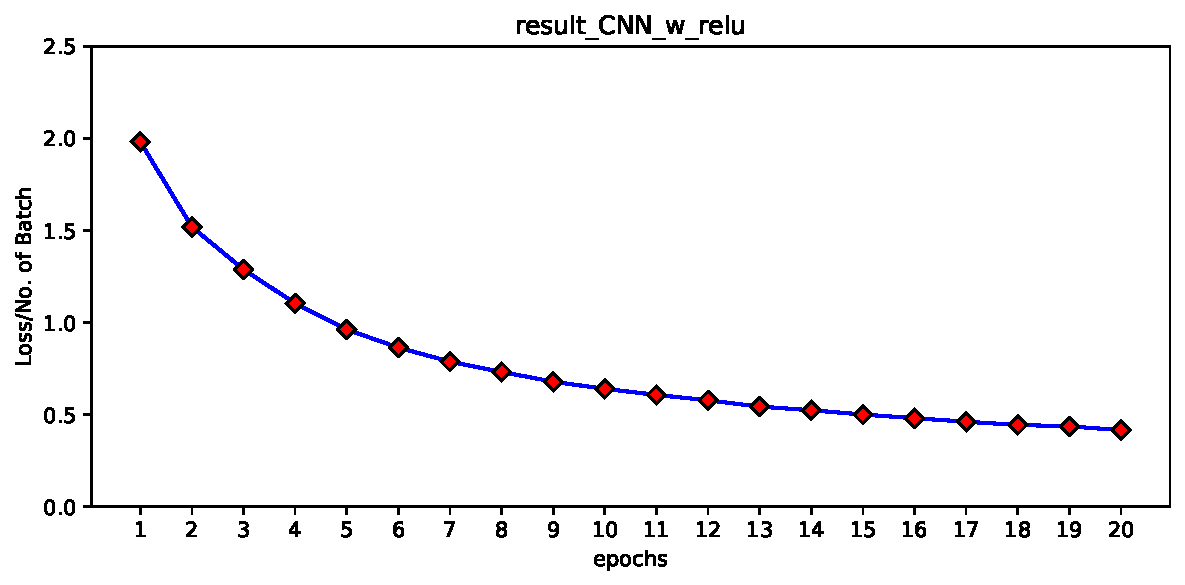
\includegraphics[width=0.45\textwidth]{./results/result_CNN_w_relu.pdf}%
      \label{fig:cnn_loss}
   }%
   % \label{fig:llr_sgd}
   \hspace{0.5cm}%
   \subfloat[][CNN Accuracy]
   {%
      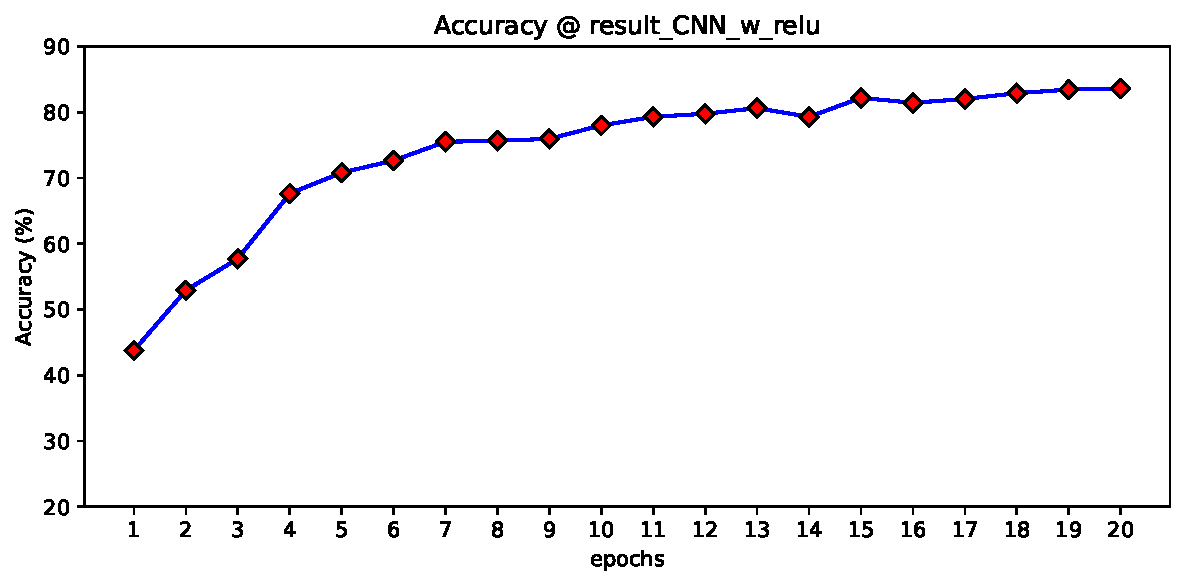
\includegraphics[width=0.45\textwidth]{./results/result_CNN_w_relu_accuracy.pdf}%
      \label{fig:cnn_acc}
   }
   \caption{Convolutional Neural Network training results.}
\end{figure}
\vspace*{-0.6cm}
\section*{On MLP v. CNN}
\vspace*{-0.4cm}
The difference in the performance of the two models are obvious.
From the reported training results, it could be seen that CNN has a superior
model accuracy, where it reaches around $85 \%$, where MLP only achieves $50 \%$,
while having less loss.
With a same training epochs, MLP was trained faster with 267 seconds,
whereas CNN was with 308.
\vspace*{-0.6cm}
\section*{NNs without Activation Layers}
\vspace*{-0.4cm}
The last section presents the training results when we remove the activation layers,
i.e., ReLU in this case. Below first presents training results of the two.

Multi-Layer Perceptron:
\begin{figure}[!htb]
   \captionsetup[subfigure]{justification=centering}
   \centering
   \subfloat[][MLP (no ReLU) Loss v. Epochs]
   {%
      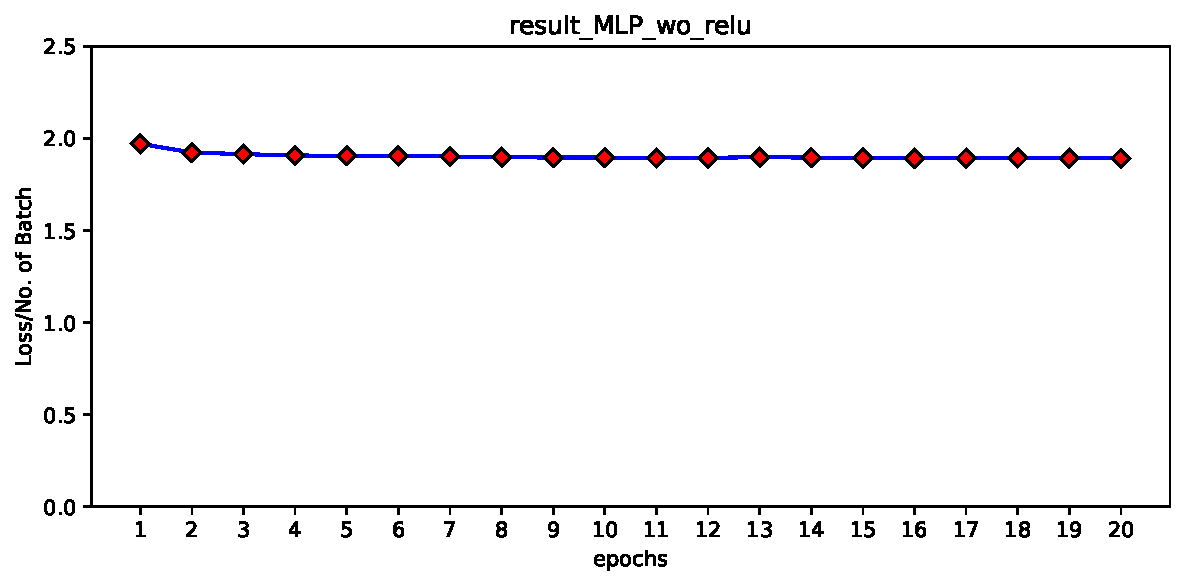
\includegraphics[width=0.45\textwidth]{./results/result_MLP_wo_relu.pdf}%
      \label{fig:mlp_norelu_loss}
   }%
   % \label{fig:llr_sgd}
   \hspace{0.5cm}%
   \subfloat[][MLP (no ReLU) Accuracy]
   {%
      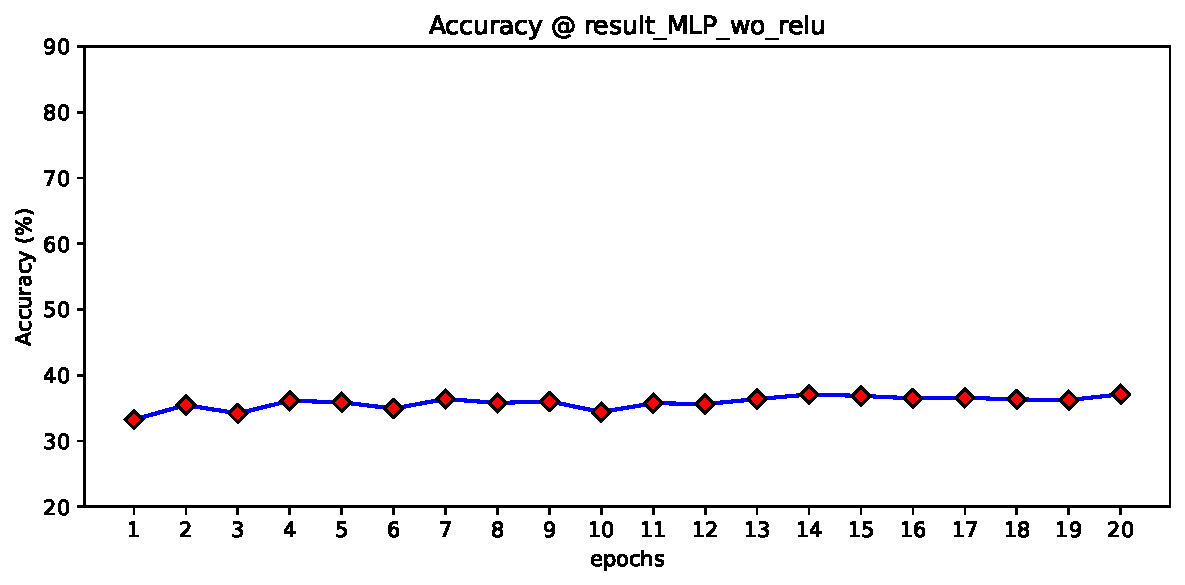
\includegraphics[width=0.45\textwidth]{./results/result_MLP_wo_relu_accuracy.pdf}%
      \label{fig:mlp_norelu_acc}
   }
   \caption{Multi-Layer Perceptron with no activation layer training results.}
\end{figure}

Convolutional Neural Network:
\begin{figure}[!htb]
   \captionsetup[subfigure]{justification=centering}
   \centering
   \subfloat[][CNN (no ReLU) Loss v. Epochs]
   {%
      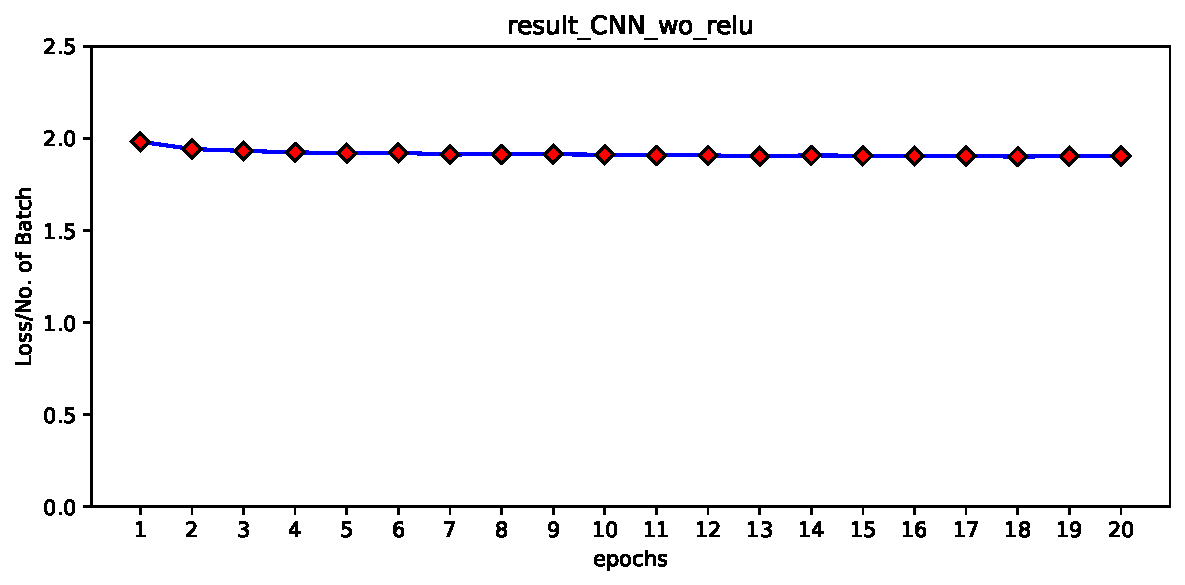
\includegraphics[width=0.45\textwidth]{./results/result_CNN_wo_relu.pdf}%
      \label{fig:cnn_norelu_loss}
   }%
   % \label{fig:llr_sgd}
   \hspace{0.5cm}%
   \subfloat[][CNN (no ReLU) Accuracy]
   {%
      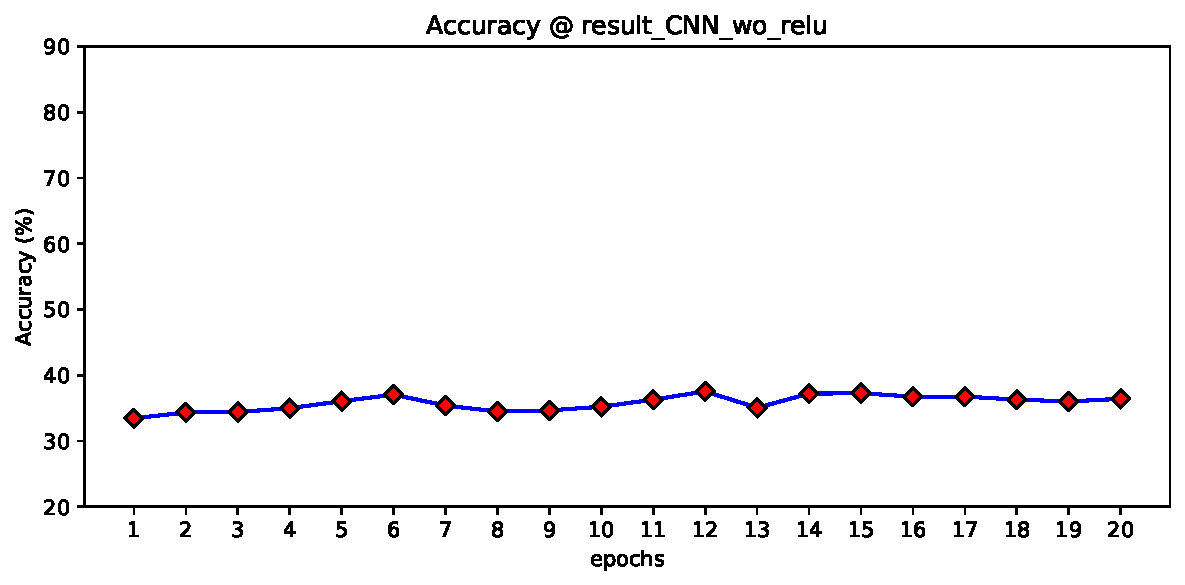
\includegraphics[width=0.45\textwidth]{./results/result_CNN_wo_relu_accuracy.pdf}%
      \label{fig:cnn_norelu_acc}
   }
   \caption{Convolutional Neural Network with no activation layer training results.}
\end{figure}

From above, as observed, without the activation layers, the performance drops drastically
in both MLP and CNN. 
The main reason behind this due to the fact that, without the nonlinearity induced
by ReLU, the models are simply linear. 
Training the two models with such settings could therefore be seen as a linear regression
models with a higher dimension.
And therefore, that is why although CNN achieves higher accuracy in the original settings,
under the circumstances where the ReLU layers were removed, it behaves as poorly as MLP, 
achieving an accuracy between 30 \% and 40 \%.



\bibliographystyle{IEEEtran}
% \bibliography{references}

\end{document}

